% Chapter 1

\chapter{Introduction} % Main chapter title

\label{Chapter1} % For referencing the chapter elsewhere, use \ref{Chapter1} 

%----------------------------------------------------------------------------------------

% Define some commands to keep the formatting separated from the content 
\newcommand{\keyword}[1]{\textbf{#1}}
\newcommand{\tabhead}[1]{\textbf{#1}}
\newcommand{\code}[1]{\texttt{#1}}
\newcommand{\file}[1]{\texttt{\bfseries#1}}
\newcommand{\option}[1]{\texttt{\itshape#1}}






%1----------------------------------------------------------------------------------------



\section{Contexte}



Le déclin de la glace Artique ces dernières décenies est considéré comme l'une manifestations les plus marquante du changement climatique (voir \parencite{stroeve2012trends}). Ce déclin présente des enjeux aussi climatiques qu'industriels. Premièrement, de par son étendue et son epaisseur immense, la la zone artique est un contributeur majeur climat à travers ses échanges de chaleurs par rayonnement et radiation avec l'atmosphère. Il est donc crucial de considérer l'évolution de la glace dans les modèles climatiques. Deuxièmement, la chute de cette couverture de glace dans la MIZ\footnote{Marginal Ice Zone : zone de transition entre l’océan et le coeur de la banquise, où la concentration de
glace est inférieure à 80\%, et/ou les morceaux de glace sont de faible épaisseur ($\approx 1 mètre$) et de petite taille ($10 m - 100 km$).} (voir \cref{fig:miz}) ouvre des routes maritimes facilitant l'exploitation de ses réserves d’hydrocarbures (qui restent quasiment intactes). Il est donc nécéssaire de pouvoir prédire l'évolution de la banquise Artique (au moins) à court terme.


Parmis les élément exhaxerbant ce déclin de galce Artique, des études ont cité l'accélération de la vitesse et de la déformation des floes\footnote{Un floe est un morceau indiviiduel de glace rencontré dans la MIZ} (RWDC11, SKM11). Pour les prédiction de l'évolution de la banquise, les modèles qui considère la glace comme un milieu continu ne sont pas adapté, surtout à l'échelle de la MIZ. Au contraire, les modèle granulaire, bien que plus couteux doivent etre priviligé afin de prendre en compte la nature discontinue de la banquise et sa rhéologie\footnote{étudie la résistance des matériaux aux contraintes et aux déformations.}. Des modèles granulaires pour l'évolution de la glace ont été utilisés par le passé (Hop96, KS14). Cependant, les approches utulisées dans ces travaux limitent la géométrie (circulaire, rectangulaire) et le nombre de floes (de l'ordre de la centaine) et modélisent donc le contact entre floes comme une répulsion après interpénétration\footnote{Les détails sur l'interpénétration sont donnés à la ... } (voir \parencite[p.16]{balasoiu2020halthesis}). 

En 2015, M. Rabatel, S. Labbé et J. Weiss \parencite{rabatel2015dynamics,rabatel2015thesis} ont développé un nouveau modèle granulaire prenant en compte la collision des floes sans passer par un processus d’interpénétration (voir \cref{fig:simugranu1}). Dans leur modèle, le mouvement des floes vérifie les équations de préservation du moment angulaire et de la quantité de mouvement. Le modèle prend en compte la force de Coriolis et les interactions avec l’océan et l’atmosphère. En 2020, D. Balasoiu \parencite{balasoiu2020halthesis} développe un modèle de fracture dans le but de le coupler au modèle granulaire d'interaction préexistant, en prenant en compte le phénomène de percussion\footnote{Dans ce rapport, nous désignerons par percussion la série de collision à très courts intervalles de temps entre deux ou plusieurs floes.}. Les floes de glace auparavant considérés comme des corps solides dans les travaux de M. Rabatel, sont dorénavant des coprs élastiques. En plus de proposer un modèle de fracture fragile pour les floes de glace, D. Balasoiu obtient l’expression du déplacement d'un floe (cette fois ci considéré comme un réseau de masses-ressorts-dispositifs visqueux) qui est percuté par object pontuel.

C'est dans ce contexte que le projet SASIP a été lancé. Il s'agit d'un projet a but de developper un nouvea modèle de glace de mer capable d'appréhender sa dynamique complexe afin d'améiorer sa représentation dans les futurs modèles de pr'diction climatiques. Cette gigantesque entreprise pilotée par l'Institut des Géosciences de l'Environnement regroupe dix partenaires internationaux parmi lesquels la France, la Norvège, les Etats-Unis d'Amérique, l'Italie, le Royaume Unis, et l'Allemagne. Ce fut un grand honneur pour mois d'intégré ce projet dans un stage de six mois avec pour missions: prendre en main puis de poursuivre le développement du modèle de fracturation des floes existant; intégrer ce modèle dans un code de calcul de l’évolution de la banquise à l’échelle des floes de glace.


\begin{figure}[!h]
    \centering
    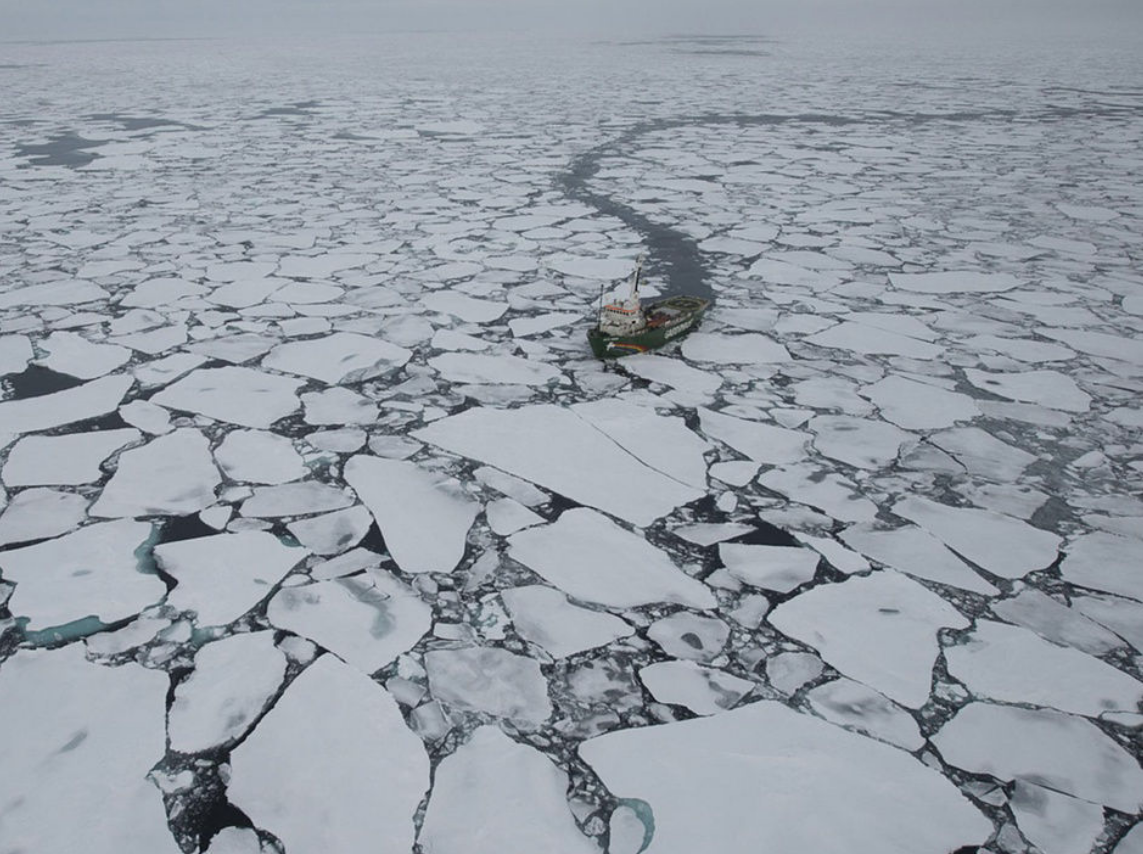
\includegraphics[width=0.55\textwidth]{IceRoutes.png}
    \caption{Un bateau industriel dans la Marginal Ice Zone (MIZ).}
    \label{fig:miz}
\end{figure}

\begin{figure}[!h]
    \centering
    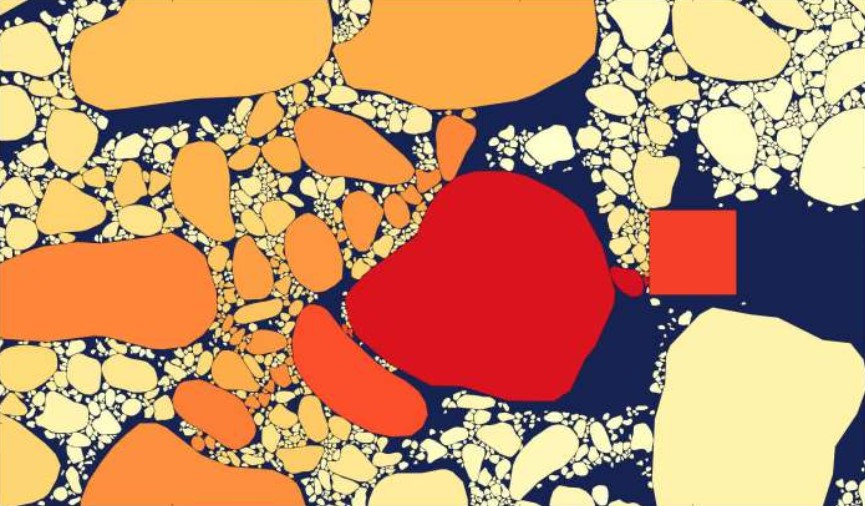
\includegraphics[width=0.65\textwidth]{SimuGranu1.jpg}
    \caption{Capture d’écran d’une simulation d’interaction glace structure avec contact rigide \parencite[p.23]{balasoiu2020halthesis}.}
    \label{fig:simugranu1}
\end{figure}


%2----------------------------------------------------------------------------------------





\section{Problématique}


Ce stage a été pour moi une opportunité d'explorer la percussion et la fracture des floes de glace. J'ai eu à développer un modèle mathématique et à l'intéger à un projet de développement logiciel. Plus précisément, ce rapport de stage se développe au prisme de la problématique du composrtement d'un matériaux élastique lors de la percussion avec un matériaux voisin. En utilisant les principes de mécanique du contact et les équation aux dérivées ordianaires (EDO), nous nous sommes intérrésés à la question: \emph{Comment le matériau se déplace-t-il après de tel(s) choc(s)?} Nous nous somme aussi posé la question de savoir \emph{dans quelle mesure une fracrure apparait-t-elle dans le matériau?} Pour cette dernière tache, nous nous sommes basés sur le modèle de Griffith et de l'approche de Franckfort-Marigot.






%3----------------------------------------------------------------------------------------





\section{Environnement}


Mon stage s'est déroulé du 02 février au 31 juillet 2021 au sein du Laboratoire Jacques Louis Lions (LJLL) de Sorbonne Université, sous la supervision du Professeur Stéphane Labbé. Ce stage s'incirt dans la continuation directe de deux thèses effectuée par Matthias Rabatel \Parencite{rabatel2015thesis} et Dimitri Balasiou \parencite{balasoiu2020halthesis} au sein du Laboratoire Jean Kuntzmann de l'Université Grenoble Alpes, co-dirigées par le Professeur Stéphane Labbé, et Monsieur Jérôme Weiss, en colaboration avec le groupe TOTAL. Le LJLL a consituté un environnement idéal pour ce travail de stage de par ses membres spécialées dans divers domaines des mathématiques appliquées, et des ressources mises à ma disposition pour le remplissage de mes fonctions. Cependant, malgré la convivialité et l'esprit d'équipe reignant au sein du LJLL, j'ai  du effectué certaines de mes taches en télétravail principalement du à la situation de confinnement imposée en France durant cette période trouble de pandémie liée à la COVID-19.



%4----------------------------------------------------------------------------------------





\section{Objectifs}
\label{sec:introobk}

Au vue des problème qui nous sont donné de résoudre et des travaux qui ont précédés, nos \emph{objectifs primaires} de ce rapport de stage (ainsi que leur temps approximatif d'exécution) sont les suivants:
\begin{enumerate}
    \item Comprendre le modèle de rupture de Griffith dans les milieux élastiques (6 semaines).
    \item Comprendre le passage micro/macro du modèle élastique pour travailler sur le modèle de percussion. 
    \item Intégrer le modèle dans un code de calcul de l’évolution
    de la banquise à l’échelle des floes de glace.
\end{enumerate}

Afin de remplir au miieux ces missions, nous les avons fracturé en groupes de taches singulières formant ainsi des \emph{objectifs secondaires} étalé sur six mois (26 semaines) que sont:   

\begin{itemize}
    \item Prise en main de la notion de Gamma-Convergence en calcul des variations (effectuée avant le début du stage)
    \item Lecture et assimilation de la thèse de Matthias Rabatel (jusqu'au 23 février 2021)
    \item Lecture et assimilation de la thèse de Dimitri Balasoiu (jusqu'au 16 février 2021)
    \item Modéliser, simuler, et visualiser le déplacement d'un floe en une dimension (1D) après une collision (jusqu'au 30 mai 2021)
    \item Modéliser, simuler, et visualiser le déplacement d'un floe en deux dimension (2D) après une collision (jusqu'au 30 juin 2021)
    \item Implémenter le modèle de fracture de Griffith dans le modèle de collision 1D préexistant (30 juillet 2021)
\end{itemize}



En vue de rendre compte de manière fidèle et analytique des six mois passés au sein du Laboratoire Jacques-Louis Lions, il apparaît logique de présenter à titre préalable les remarquables travaux qui ont précédé ce stage (\cref{Chapter2}); puis de présenter les différents modèles de glace de mer développés et étudiés en 1D (\cref{Chapter3}); ensuite en 2D (\cref{Chapter4}). Enfin, à l'aide d'un journal de bord, il sera précisé les différentes tâches que j’ai pu effectuer, et les nombreux apports que j’ai pu en tirer (\cref{Chapter5}). 





%5----------------------------------------------------------------------------------------




\section{Abstract}


The rapid shrinking of the Artic ice cap these last decades is considered as one of the most striking manifestations of global warming \parencite{stroeve2012trends}. The decrease in size open way to new opportunities. Namely ice routes benefical to the indistrial sector. The second major consequence is these studies is the necessity to include the MIZ into climate prediction models. In 2015, Rabatel et al. \parencite{rabatel2015dynamics,rabatel2015thesis} developped a sophiticated model for the dynamics of rigid ice floes. The model was later enhanced by Balasoui in 2020 when he considered the ice floes not as rigid, but as elastic materials easily modeled by a mass-spring-damper lattice \parencite{balasoiu2020halthesis}. Our goal is to introduce the fracture into this model. Specificaly, we will study what happens when two or more ice floes collide (percussion, fracture, etc.) both in 1D and in 2D.